\documentclass[tikz,border=8pt]{standalone}
% Shared look for every TikZ diagram. Load with % Shared look for every TikZ diagram. Load with % Shared look for every TikZ diagram. Load with \input{../../tools/tikz-style.tex}
\usepackage[T1]{fontenc}
\usepackage{lmodern}
\renewcommand{\sfdefault}{lmr}  % diagrams use the same serif as the text
\usetikzlibrary{arrows.meta, positioning, shapes.geometric, calc, fit, backgrounds}
\definecolor{cblue}{HTML}{4C78A8}
\definecolor{corange}{HTML}{F58518}
\definecolor{cgreen}{HTML}{54A24B}
\definecolor{cred}{HTML}{E45756}
\definecolor{cpurple}{HTML}{B279A2}
\definecolor{cgrey}{HTML}{6B6B6B}
\tikzset{
  every picture/.style={font=\sffamily, line width=1.2pt},
  box/.style={draw=#1, fill=#1!12, rounded corners=4pt, align=center, inner sep=7pt, minimum height=1.1cm},
  box/.default=cgrey,
  arrow/.style={-{Stealth[length=3mm]}, draw=cgrey, line width=1.4pt},
  title/.style={font=\sffamily\bfseries\Large},
  note/.style={font=\sffamily\small, text=cgrey, align=center},
}
\AtBeginDocument{\hyphenpenalty=10000 \exhyphenpenalty=10000}

\usepackage[T1]{fontenc}
\usepackage{lmodern}
\renewcommand{\sfdefault}{lmr}  % diagrams use the same serif as the text
\usetikzlibrary{arrows.meta, positioning, shapes.geometric, calc, fit, backgrounds}
\definecolor{cblue}{HTML}{4C78A8}
\definecolor{corange}{HTML}{F58518}
\definecolor{cgreen}{HTML}{54A24B}
\definecolor{cred}{HTML}{E45756}
\definecolor{cpurple}{HTML}{B279A2}
\definecolor{cgrey}{HTML}{6B6B6B}
\tikzset{
  every picture/.style={font=\sffamily, line width=1.2pt},
  box/.style={draw=#1, fill=#1!12, rounded corners=4pt, align=center, inner sep=7pt, minimum height=1.1cm},
  box/.default=cgrey,
  arrow/.style={-{Stealth[length=3mm]}, draw=cgrey, line width=1.4pt},
  title/.style={font=\sffamily\bfseries\Large},
  note/.style={font=\sffamily\small, text=cgrey, align=center},
}
\AtBeginDocument{\hyphenpenalty=10000 \exhyphenpenalty=10000}

\usepackage[T1]{fontenc}
\usepackage{lmodern}
\renewcommand{\sfdefault}{lmr}  % diagrams use the same serif as the text
\usetikzlibrary{arrows.meta, positioning, shapes.geometric, calc, fit, backgrounds}
\definecolor{cblue}{HTML}{4C78A8}
\definecolor{corange}{HTML}{F58518}
\definecolor{cgreen}{HTML}{54A24B}
\definecolor{cred}{HTML}{E45756}
\definecolor{cpurple}{HTML}{B279A2}
\definecolor{cgrey}{HTML}{6B6B6B}
\tikzset{
  every picture/.style={font=\sffamily, line width=1.2pt},
  box/.style={draw=#1, fill=#1!12, rounded corners=4pt, align=center, inner sep=7pt, minimum height=1.1cm},
  box/.default=cgrey,
  arrow/.style={-{Stealth[length=3mm]}, draw=cgrey, line width=1.4pt},
  title/.style={font=\sffamily\bfseries\Large},
  note/.style={font=\sffamily\small, text=cgrey, align=center},
}
\AtBeginDocument{\hyphenpenalty=10000 \exhyphenpenalty=10000}

\begin{document}
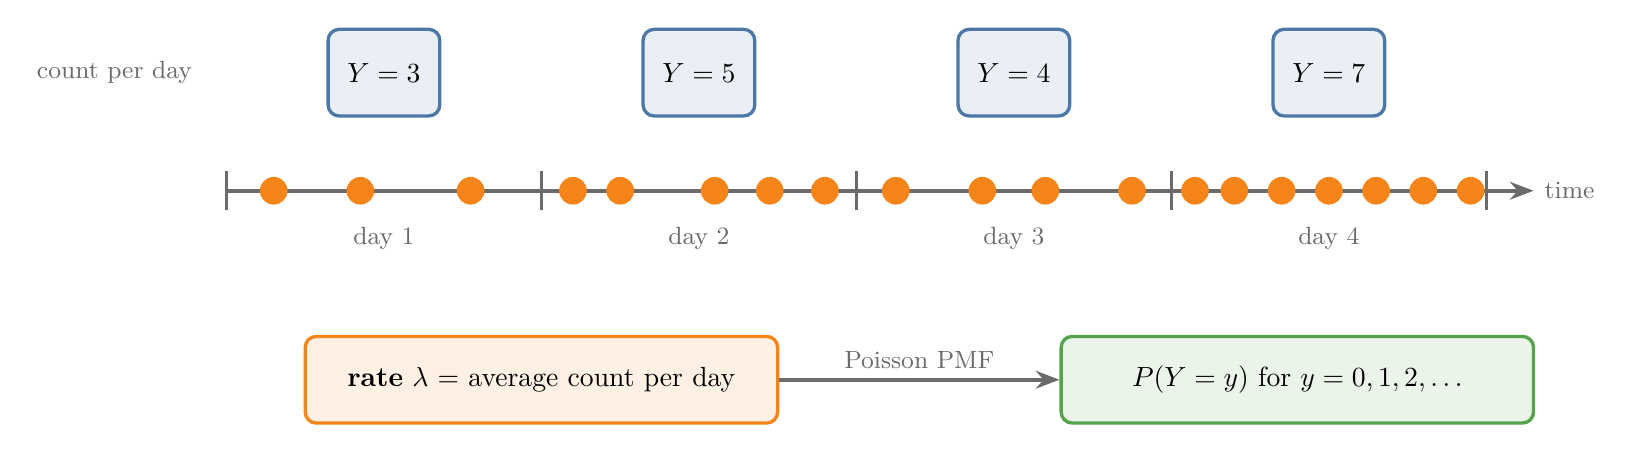
\begin{tikzpicture}
  % a time line split into four equal intervals (days); each dot is one event (a question)
  \draw[cgrey, line width=1.4pt, -{Stealth[length=3mm]}] (0,0) -- (16.6,0) node[right, note] {time};
  \foreach \x in {0,4,8,12,16} \draw[cgrey] (\x,-0.25) -- (\x,0.25);
  \foreach \d/\lab in {0/day 1,4/day 2,8/day 3,12/day 4} \node[note] at (\d+2,-0.6) {\lab};
  % event positions inside each day
  \foreach \x in {0.6,1.7,3.1} \fill[corange] (\x,0) circle (5pt);
  \foreach \x in {4.4,5.0,6.2,6.9,7.6} \fill[corange] (\x,0) circle (5pt);
  \foreach \x in {8.5,9.6,10.4,11.5} \fill[corange] (\x,0) circle (5pt);
  \foreach \x in {12.3,12.8,13.4,14.0,14.6,15.2,15.8} \fill[corange] (\x,0) circle (5pt);
  % counts
  \foreach \d/\c in {0/3,4/5,8/4,12/7} \node[box=cblue, minimum width=1.2cm] at (\d+2,1.5) {$Y = \c$};
  \node[note, anchor=east] at (-0.3,1.5) {count per day};
  % summary
  \node[box=corange, minimum width=6cm] (lam) at (4,-2.4) {\textbf{rate} $\lambda$ = average count per day};
  \node[box=cgreen, minimum width=6cm] (q) at (13.6,-2.4) {$P(Y = y)$ for $y = 0, 1, 2, \dots$};
  \draw[arrow] (lam) -- (q) node[midway, above, note] {Poisson PMF};
\end{tikzpicture}
\end{document}
